\documentclass{report}

\usepackage{graphicx}
\usepackage{cancel}
\usepackage{amsmath}
\usepackage{ragged2e}

\usepackage{nopageno}
\usepackage[utf8]{inputenc}
\usepackage[english,russian]{babel}
\usepackage[a4paper, left=0.4cm, top=0.5cm, right=0.4cm, bottom=0.5cm]{geometry}




\begin{document}


\noindent
\textbf{Векторная функция} векторного аргумента -- это соответствие $r$, при котором
$\forall$ точке $x \in \Omega$ евклидова пространства $R^{m}$ сопостовляется 
вектор $r(x)$ множества $Q$ евклидова пространства $R^{p}$.\\
$x \in \Omega = \{(x_1, \ldots, x_m)\} \subset R^{m} \to r(x)
\in Q = \{(r_1, \ldots, r_p)\} \subset R^{p}$\\
При этом множество $\Omega$ область задания, а $Q$ множество значений.
Если $\Omega = \{x\}$ -- множество точек на прямой, то имеем функцию одного
скалярного аргумента $r(x)$.\\
Если $\Omega = \{(x_1, \ldots, x_m)\} \subset R^{m}$ -- множество точек евклидова
пространства, то имеем векторную функцию нескольких скалярных
аргументов $r(x_1, \ldots, x_m)$.\\

\noindent
\textbf{Годограф векторной функции}\\
Пусть $(r_1, \ldots, r_p)$ -- координаты $r(x) \in Q \subset R^{p}$.
Задание векторной функции $r(x)$ равносильно заданию скалярных функций\\
$r_1(x_1, \ldots, x_m), \ldots, r_p(x_1, \ldots, x_m)$, и если начала этих
векторов совместить с началом соответствующей ДПСК, то точечное множество концов
рассматриваемых радиус векторов будем называть годографом векторной функции.\\
If p = 3 годограф векторной функции есть кривая, p = 2 -- поверхность.\\


\noindent
\textbf{Способы задания кривых}\\
\indent Элементарной кривой называют множество точек пространства, являющееся
образом отрезка при топологическом отображении его в пространство.\\
Точки соответствующие конечным точкам отрезка, называют конечными точками
элементарной кривой. Элементарные кривые -- примыкающие если одна или обе
пары их конечных точек совпадают между собой.\\
Кривой линией называется множество точек пространства, которое состоит
из конечного или счетного множества элементарных кривых, примыкающих друг к другу.\\
\indent Пусть $\gamma$ -- элементарная кривая, являющаяся образом промежутка 
$a < t < b$ при топологическом отображении f его в пространство $R^{3}$.
$x(t),\ y(t),\ z(t)$ -- координаты точки на кривой $\gamma$ соответствующей
значению $t \in (a, b)$.\\
Тогда систему равенств $x(t),\ y(t),\ z(t),\ t \in (a, b)$ называют уравнениями кривой 
$\gamma$ в параметрической форме или параметризацией кривой (кривая $\gamma$ параметризована
этими уравнениями).\\
Если же считать $x(t),\ y(t),\ z(t)$ координатами радиус-вектора $\overrightarrow{r}(t)$
соответствующей точки кривой $\gamma$, мы получим векторную функцию $\overrightarrow{r}(t),\ $
$t \in (a, b)$, годографом которой является данная кривая. (способ задания кривой через векторную
функцию скалярного аргумента по сути эквивалентный параметрическому способу).\\
Допустим, что кривая $\gamma$ задается векторной функцией $\overrightarrow{r}(t),\ t \in (a, b)$.\\
Тогда заменив параметр $t$ параметром $u$ через отношение $t = g(u),\ u \in (\alpha, \beta),$ где $g$
-- строго возрастающая и непрерывная функция. Тогда получится новая параметризация, одну кривую
можно задать множеством параметризаций.\\
Гладкая кривая -- такая кривая, у которой векторная функция
с помощью которой задана кривая дифференциируема 1 раз.
Регулярная $k$ раз $k \geq 1$.\\

\noindent
\textbf{Касательная к кривой}\\
Пусть $\gamma$ -- некторая кривая, $P$ -- фиксированная точка и $M$ -- подвижная точка на кривой
$\gamma,\ PM$ -- хорда кривой.\\
Прямая $PM$ стремится к прямой $PT$ при $M \to P$, если угол $\varphi$ между этими прямыми стремится
к нулю, когда $M \to P$.\\
Касательной к кривой $\gamma$ в точке $P$ называют прямую $PT$, к которой стремится хорда $PM$,
когда $M \to P$.\\
\begin{figure}[ht!]
\centering
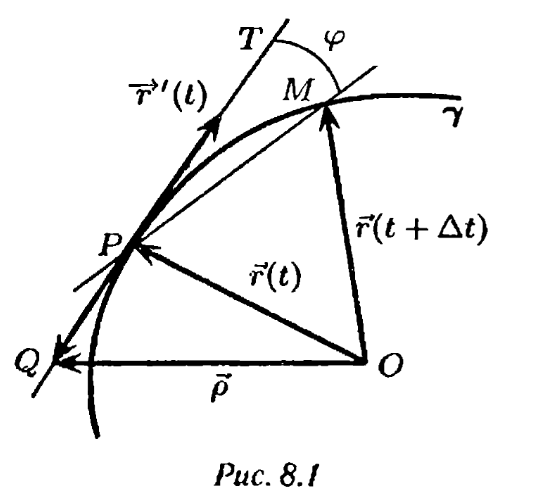
\includegraphics[width=60mm]{curve.png}
\end{figure}

\noindent
\textbf{Нормальной плоскостью кривой} в точке $P$ называется плоскость, проходящая через точку
$P$ перпендикулярно касательной в данной точке.\\
Векторное уравнение нормальной плоскости $\pi$ в точке $P(\overrightarrow{r}(t))$ имеет вид:
$(\overrightarrow{\rho} - \overrightarrow{r}(t)) \cdot \overrightarrow{r}'(t) = 0$, где 
$\overrightarrow{\rho}$ -- радиус-вектор произвольной точки плоскости $\pi$.\\

\newpage
\noindent
\textbf{Соприкасающаяся плоскость}\\
Пусть $\gamma$ -- некоторая кривая, $P \in \gamma$ -- фиксированная точка, $M \in \gamma$ --
подвижная, $PT$ -- касательная к кривой в точке $P$, $PTM$ -- плоскость проведенная через
касательную $PT$ и точку $M$.\\
Плоскость $RTM$ стремится к плоскости $\pi$ при $M \to P$, если угол между этими плоскостями
стремится к нулю, когда $M \to P$.\\
Плоскость $\pi$, к которой стремится плоскость $PTM$, когда $M \to P$, называют
соприкасающейся плоскостью кривой $\gamma$ в точке $P$.\\
\begin{figure}[ht!]
\centering
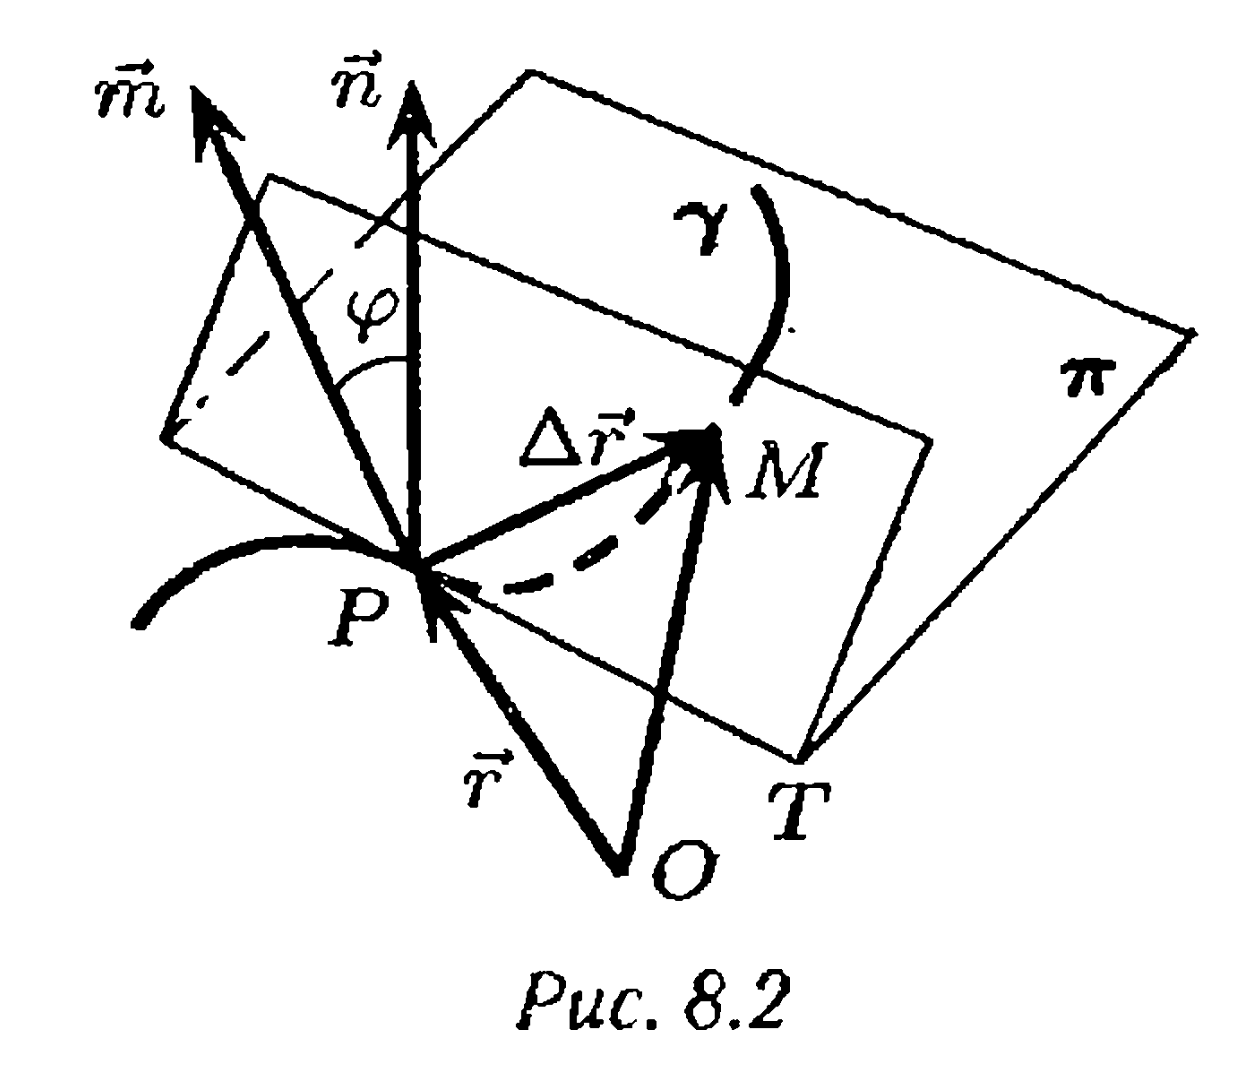
\includegraphics[width=60mm]{curve2.png}
\end{figure}


\noindent
\textbf{Спрямляющая плоскость, главная нормаль, бинормаль}\\
Прямую проходящую через точку $P$ перпендикулярно касательной кривой,
называют нормалью кривой. $(CD, MN)$\\ 
Нормаль, лежащую в соприкасающейся плоскости кривой,
называют главной нормалью кривой. $(CD)$\\
Нормаль, перпендикулярную соприкасающейся плоскости кривой,
называют бинормалью кривой. $(MN)$\\
Плоскость, определяемую касательной к кривой и бинормалью, 
называют спрямляющей плоскостью. $(\pi_3)$\\
\begin{figure}[ht!]
\centering
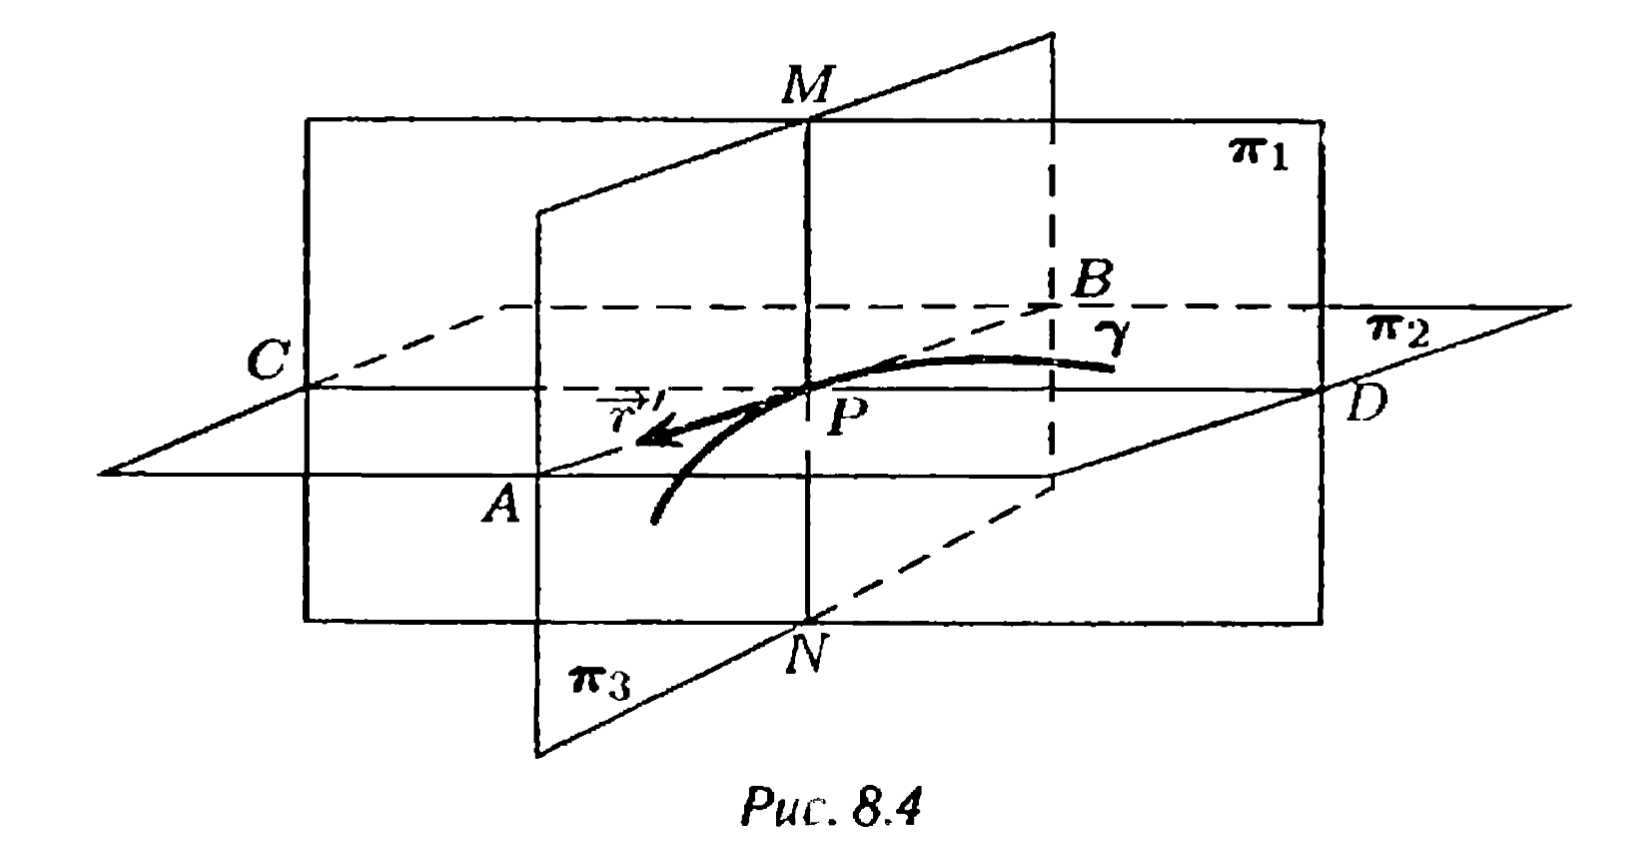
\includegraphics[width=90mm]{curve3.png}
\end{figure}


\noindent
\textbf{Длина дуги кривой}\\
Пусть $\gamma = \buildrel\, \, \frown\over{AB}$ -- дуга кривой, являющаяся образом замкнутого отрезка
$[a, b]$ при топологическом отображении.\\
Разобьем дугу $AB$ на $n$ частичных дуг точками: $A = A_0, \ldots, A_n = B$ и впишем в неё ломаную
с вершинами в этих точках, причем каждое звено ломаной будет хордой соответствующей частичной дуги.\\
Длиной дуги кривой называют предел периметра ломанной линии, вписанной в данную дугу, если число
звеньев этой ломаной линии неограниченно возрастает, а длина каждого звена стремится к 0.\\
\begin{figure}[ht!]
\centering
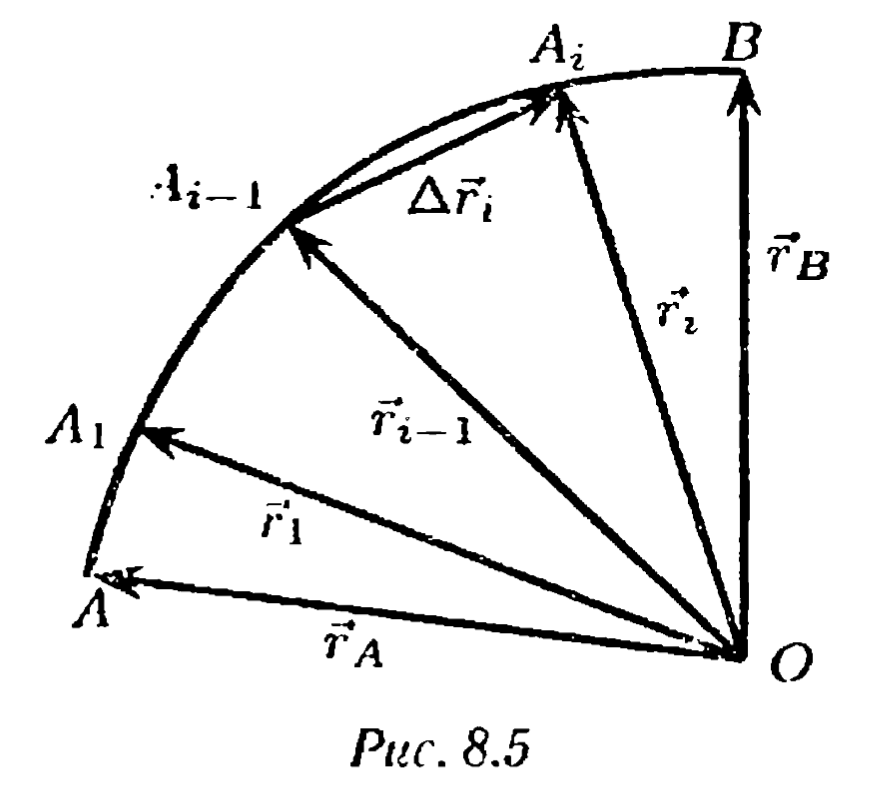
\includegraphics[width=70mm]{curve4.png}
\end{figure}


\newpage
\noindent
\textbf{Естественная параметризация}\\
Пусть $\gamma$ гладкая кривая без особых точек, $\overrightarrow{r} = \overrightarrow{r}(t)$,
$t \in (a, b)$, -- параметризация кривой $\gamma$, $J(\overrightarrow{r}(t_0))$ -- начальная
точка отвечающая параметру $t_0$.\\

\begin{figure}[ht!]
\centering
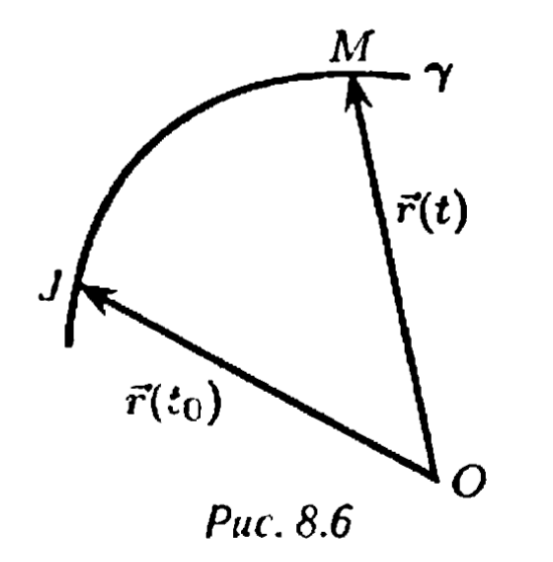
\includegraphics[width=60mm]{curve5.png}
\end{figure}

\noindent
Длина дуги имеющей начало в $J$ и конец в $M$, соотвествующей параметру $t$, определяется 
формулой $\int\limits_{t_0}^{t} |\overrightarrow{r}(t)| dt$.\\
$s(t), t \in (a, b)$ -- однозначная, дифференциируемая и монотонно возрастающая т. к. 
$\frac{ds}{dt} = |\overrightarrow{r}(t)| > 0$.\\
Значит $\exists$ обратная функция с такими же свойствами, это влечет существование 
взаимно однозначного (и непрерывного) соответствия между точками $\gamma$ и значениями длины
дуги, отсчитываемой от начальной точки $J$.\\
Точкам расположенным по разные стороны от $J$ соответствуют разные значения параметра $s$.\\
Поскольку между точками кривой $\gamma$ и значениями длины дуги $s$ $\exists$ 
взаимно однозначное и непрерывное соответствие, то длину дуги $s$ можно принять за новый
параметр, который будем называть натуральным параметром, а параметризация 
$\overrightarrow{r} = \overrightarrow{r}(s), s \in (\alpha, \beta)$, называется естественной.\\

\noindent
\textbf{Кривизна кривой}\\
Пусть $\gamma$ -- регулярная кривая без особых точек, $P \in \gamma$ -- фиксированная точка, 
$M \in \gamma$ -- точка отличная от $P$ и близкая к $P$, $\varphi$ -- угол между касательными к
$\gamma$ в точках $P, M$, $l$ -- длина дуги $\buildrel\, \, \frown\over{PM}$.\\

\begin{figure}[ht!]
\centering
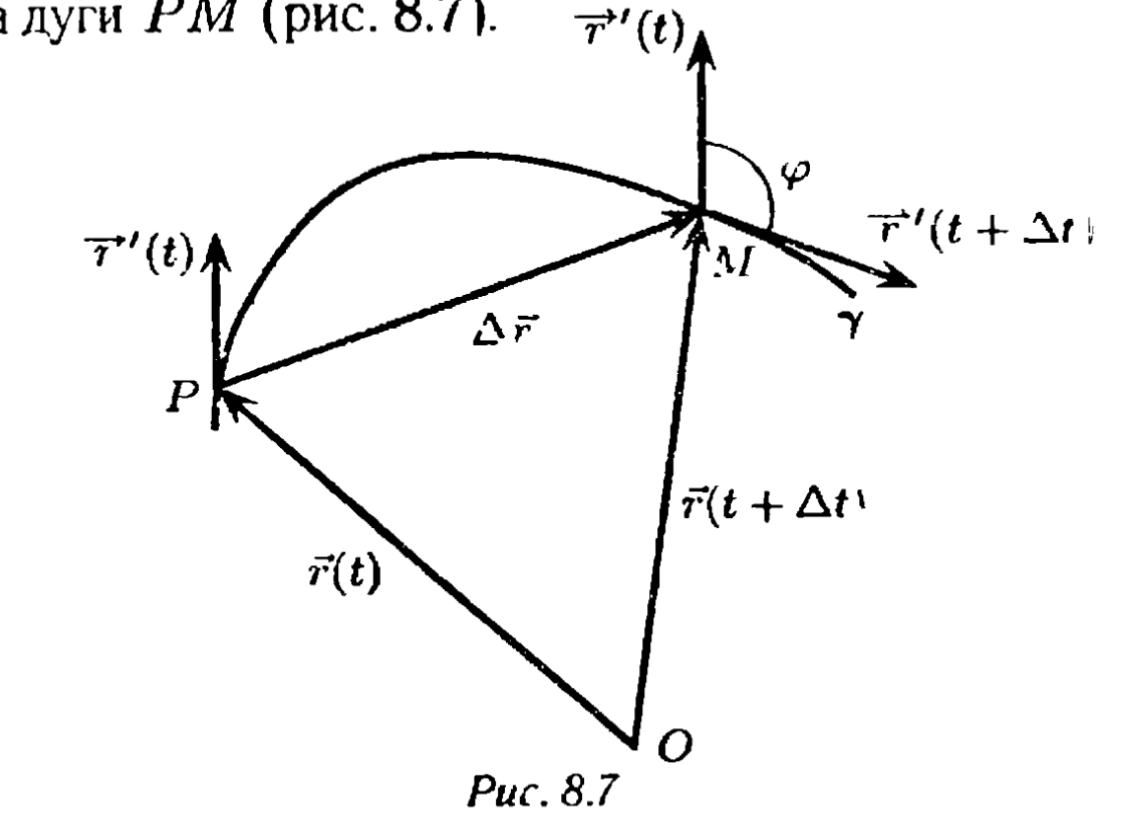
\includegraphics[width=80mm]{curve6.png}
\end{figure}

Кривизной кривой в данной точке называют передел отношения угла поворота касательной на дуге
кривой, стягивающейся к данной точке, к длине этой дуги т. е. 
$k = \lim\limits_{l \to 0}{\frac{\varphi}{l}}$.\\

\newpage
\noindent
\textbf{Кручение кривой}\\
Пусть $\gamma$ -- регулярная кривая без особых точек, $P \in \gamma$ -- фиксированная точка, 
$M \in \gamma$ -- точка отличная от $P$ и близкая к $P$, $\psi$ -- угол между
нормальными векторами $\overrightarrow{\beta}(t)$ и $\overrightarrow{\beta}(t + \delta t)$
соприкасающихся плоскостей кривой $\gamma$ в точках $P, M$, $l$ -- длина дуги
$\buildrel\, \, \frown\over{PM}$.\\

\begin{figure}[ht!]
\centering
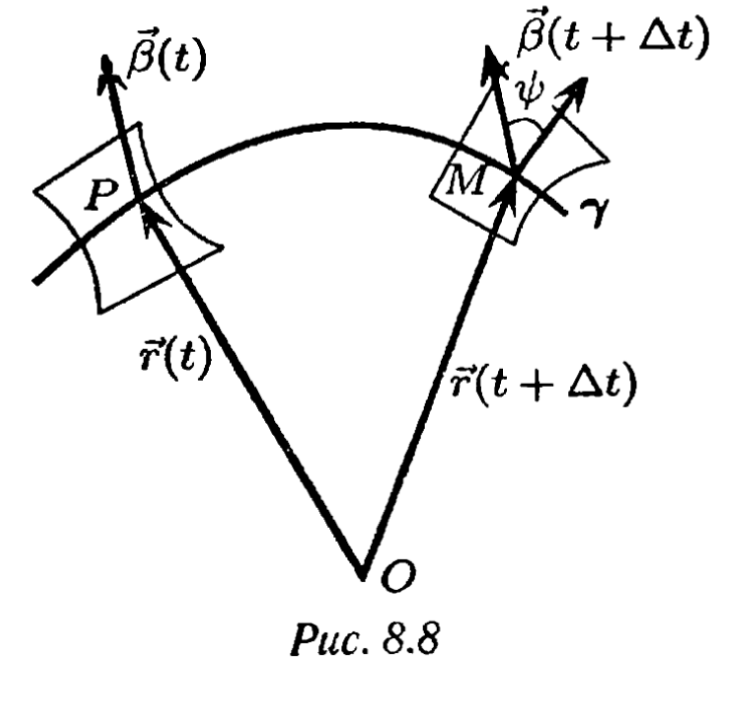
\includegraphics[width=70mm]{curve7.png}
\end{figure}

\noindent
Нормальный вектор соприкасающейся плоскости кривой лежит на бинормали
этой кривой в рассматриваемой точке.\\
Абсолютным кручением $ |\kappa| $ называют предел отношения угла поворота бинормали
на дуге кривой, стягивающейся к данной точке, к длине этой дуги: 
$ |\kappa| = \lim\limits_{l \to 0}{\frac{\psi}{l}} $\\
Если кривая задана естественной параметризацией и её кривизна 
$k(s) = |\overrightarrow{r}''(s)|, s \in (a, b)$, то абсолютное кручение в этом случае:
$|\kappa| = \frac{|(\overrightarrow{r}'(s), \overrightarrow{r}''(s), \overrightarrow{r}'''(s))|}
{k^2(s)}$.\\
Кручением кривой в точках, в которых определяется абсолютное кручение, называют величину
$\kappa(t) = \frac{(\overrightarrow{r}'(t), \overrightarrow{r}''(t), \overrightarrow{r}'''(t))}
{|\overrightarrow{r}'(t) \times \overrightarrow{r}''(t)|^2}$\\


\noindent
\textbf{Поверхность}\\
Элементарной поверхностью называют множество точек пространства, являющееся топологическим
отображением круга и ограничивающей его окружности.\\
При этом точки, являющееся топологическим отображением точек окружности, называют
граничными точками.\\
Граничные точки образуют замкнутую кривую -- границу элементарной поверхности.\\
Говорят, что две элементарные поверхности склеены, если они находятся в таком взаимном
расположении, при котором части их границ или обе границы целиком совпадают между собой.\\
Однако в результате склеивания может получиться как множество не являющееся элементарной
поверхностью так и снова элементарная поверхность.\\
Поверхностью называют множество точек пространства, которое может быть склеено из конечного
или счетного множества элементарных поверхностей.\\
Параметрическое уравнение поверхности -- $x = x(u, v), y = y(u, v), z = z(u, v), (u, v) \in D$.\\
Очевидно, что векторное уравнение будет $\overrightarrow{r} = \overrightarrow{r}(x(u, v), y(u, v),
z(u, v)), (u, v) \in D$\\

\noindent
\textbf{Координатными линиями} данной параметризации называют линии на поверхности,
соответсвующие прямым $u = const, v = const$.\\

\begin{figure}[ht!]
\centering
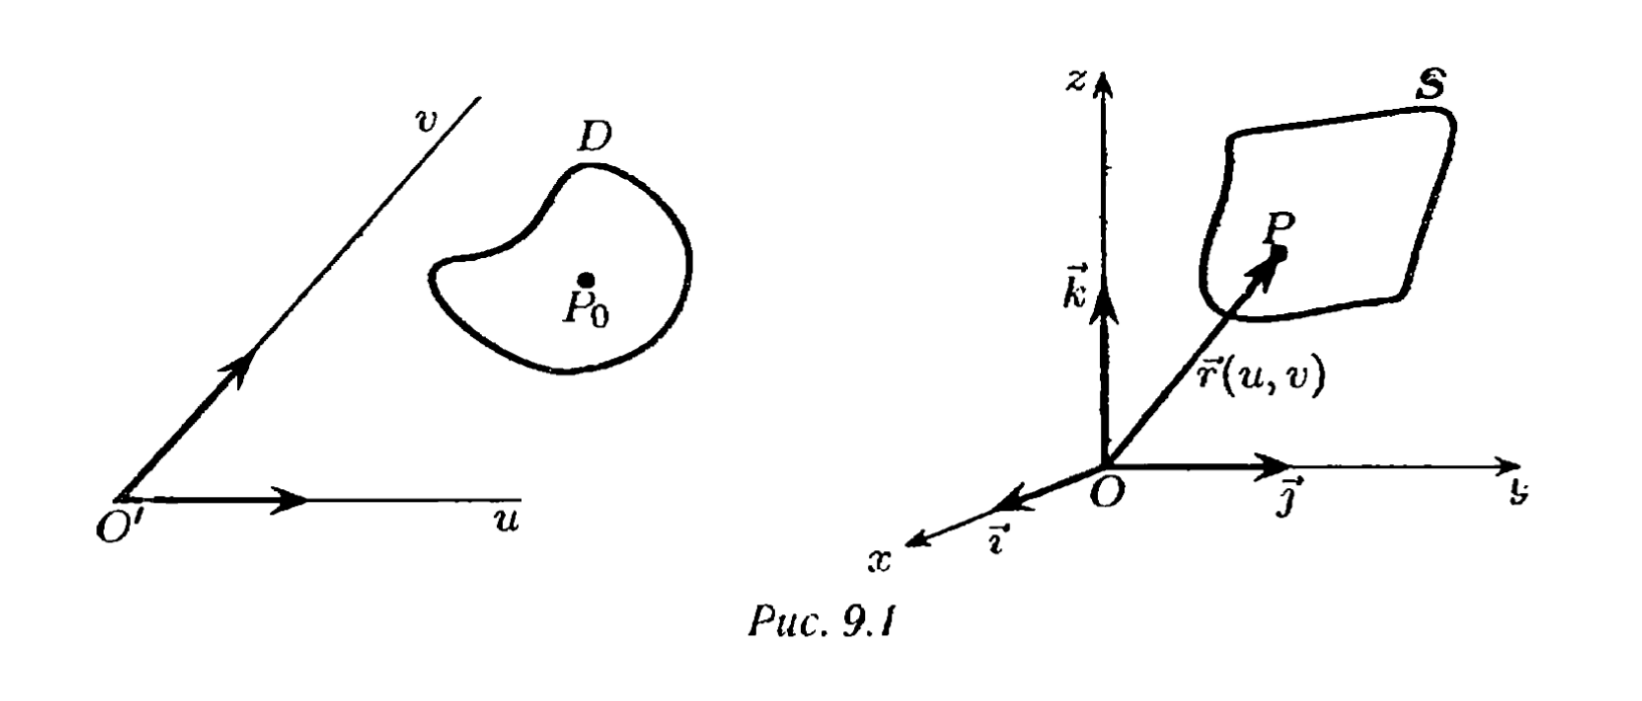
\includegraphics[width=120mm]{curve8.png}
\end{figure}

\newpage
\noindent
\textbf{Касательная плоскость}\\
Прямую называют касательной прямой к поверхности в заданной точке, если она касается
в этой точке некоторой кривой, лежащей на этой поверхности.\\
Плоскость, имеющая общую точку с поверхностью и содержащая все касательные прямые к
поверхности в рассматриваемой точке, называется касательной плоскостью к
поверхности в этой точке.\\
Уравнение касательной плоскости: 
$(\overrightarrow{\ro} - \overrightarrow{r}, \overrightarrow{r_u}, \overrightarrow{r_v}) = 0$\\

\noindent
\textbf{Нормаль к поверхности}\\
Прямую, ортогональную касательной плоскости к поверхности в данной точке и проходящую через
эту точку, называют нормалью к поверхности в указанной точке.\\
Единичный вектор нормали: $\overrightarrow{n}(u, v) = (\overrightarrow{r_u} \times
\overrightarrow{r_v})/|\overrightarrow{r_u} \times \overrightarrow{r_v}|$\\

\noindent
\textbf{Первая и вторая квадратичная форма}\\
Пусть $S$ -- регулярная поверхность без особых точек, $\overrightarrow{r} = 
\overrightarrow{r}(u, v), (u, v) \in D$, -- её векторное уравнение.\\
$\overrightarrow{n}(u, v)$ -- единичный вектор нормали поверхности в заданной точке.\\
$I = d\overrightarrow{r}^2,\ II = - d\overrightarrow{r} d\overrightarrow{n}$\\
$\to$ Первая квадратичная форма -- первая квадратичная форма дифференциалов $du, dv$\\
$I$ -- положительно определенная т. к. кроме $du = dv = 0$ всегда положительна


\end{document}
